\newpage

\begin{solution}[(Problema 1)]
    Un rectángulo como este solo puede tener un eje vertical y horizontal de simetría.
    Trazando una línea vertical y reflejando llegamos a la configuración (a).
    \begin{figure}[H]
        \centering
        \begin{subfigure}{0.27\textwidth}
            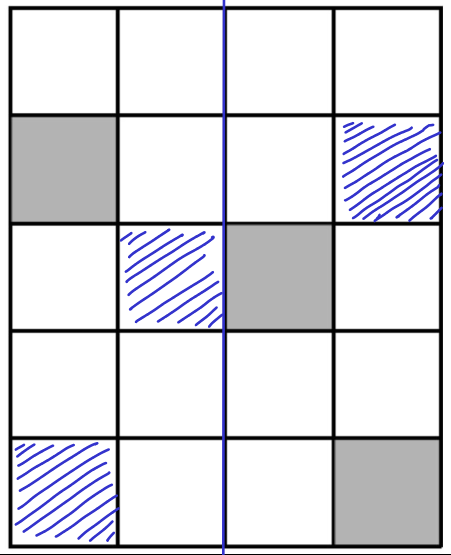
\includegraphics[width=\textwidth]{content/figure4}
            \caption{Simetría vertical}
        \end{subfigure}
        \hspace{1cm}
        \begin{subfigure}{0.27\textwidth}
            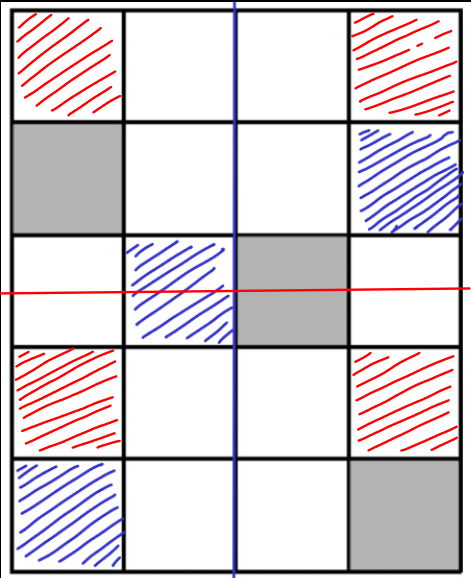
\includegraphics[width=\textwidth]{content/figure5}
            \caption{Simetría horizontal}
        \end{subfigure}
    \end{figure}
    Análogamente, tomando la configuración (a), trazando una línea horizontal y reflejando llegamos a la configuración (b).
    Luego, como mínimo se necesitan pintar 7 cuadritos más.
\end{solution}

\begin{solution}[(Problema 2)]
    Realizando la operación $m \# n = \frac{m + n}{m - n}$, sustituyendo.
    \begin{align*}
        (m\ \#\ n)\ \#\ 1 &= \left(\frac{m + n}{m - n}\right)\ \# \ 1
        = \dfrac{\frac{m + n}{m - n} + 1}{\frac{m + n}{m - n} - 1}\\
        &= \dfrac{\frac{m + n + m - n}{m - n}}{\frac{m + n- m + n}{m - n}}
        = \dfrac{\frac{2m}{m - n}}{\frac{2n}{m - n}}\\
        &= \frac{m}{n}
    \end{align*}
    Luego, se tiene que $(1\ \#\ 2025)\ \#\ 1 = \frac{1}{2025}$.
\end{solution}

\begin{solution}[(Problema 3)]
    Por dato tenemos la siguiente ecuación
    \[
        n^2 - 2n + 11 = 0.
    \]
    Convenientemente, podemos despejar $n^2 + 7 = 2n - 4 = 2(n - 2)$, multiplicando este resultado por $n$ se obtiene que
    $n^3 + 7n = 2(n^2 - 2n)$.
    Rápidamente, notamos $n^2 - 2n = -11$, usando este valor encontramos $n^3 + 7n = 2(-11) = -22$.
    Luego, al sustituir
    \[
        \frac{n^3 + 7n + 2047}{2} = \frac{-22 + 2047}{2} = \frac{2025}{2}. \qedhere
    \]
\end{solution}

\begin{solution}[(Problema 4)]
    Sea $T$ y $R$ los puntos medios de los lados $AB$ y $AC$ respectivamente, es claro que $PT = RQ = x$, por el teorema de base media
    $TR = 30$ y $AT = TB = AR = RC = 20$.
    \begin{figure}[H]
        \centering
        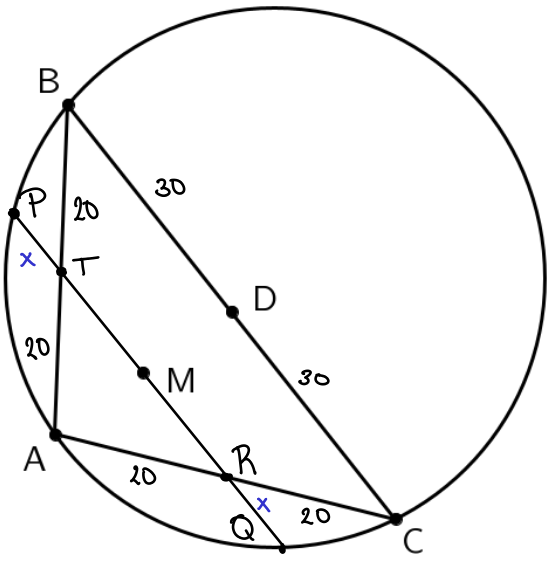
\includegraphics[width=5.8cm]{content/figure3}
    \end{figure}
    Por potencia de puntos, se tiene que $PT \cdot TQ = BT \cdot TA = 20 \cdot 20 = 400$ con lo cual $x(30 + x) = 400$,
    claramente $x = 10$ es el único valor entero positivo que cumple.
    Luego, $PQ = 10 + 30 + 10 = 50$.
\end{solution}

\begin{solution}[(Problema 5)]
    Partiremos el problema contando las veces que aparece el dígito 2 como millares, centenas, decenas y unidades.
    \begin{itemize}
        \item Para millares, solo aparecen 26 veces, esto es desde 2000 hasta 2025.
        \item Para centenas, tenemos 100 veces desde 200 a 299 y 100 veces más desde 1200 a 1299, es decir 200 veces.
        \item Para decenas, tenemos 10 veces desde 20 a 29, 10 veces desde 120 a 129, 10 veces desde 220 a 229, $\ldots$, 10 veces desde 1920 a 1929, en total $10\times 20 = 200$ veces.
        Además, 6 veces más desde 2020 a 2025, es decir 206 veces el dígito 2.
        \item Para unidades, tenemos 10 veces desde 2 a 92, 10 veces desde 102 a 192, 10 veces desde 202 a 292, $\ldots$, 10 veces desde 1902 a 1992, en total $10\times 20 = 200$ veces.
        Además, 3 veces más desde 2002 a 2022, es decir 203 veces.
    \end{itemize}
    Finalmente, la cantidad de veces que Diego escribió el dígito 2 es 26 + 200 + 206 + 203 = 635 veces.
\end{solution}

\begin{solution}[(Problema 6)]
    Sean $m$ y $n$ las cantidades de lápices y carpetas, respectivamente, por dato tenemos que $11m = 9n$.
    De esta ecuación, es claro que 9 no divide a 11, por lo cual 9 divide a $m$, por tanto $m = 9k$.
    Sustituyendo, tenemos que $11 (9k) = 9n$ lo que implica que $n = 11k$.
    Es decir, que la cantidad total de artículos está dado por $m + n = 11k + 9k = 20k$, así el problema se reduce a encontrar $k$.
    Como la cantidad total está entre 80 y 120, tenemos que $80 < 20k < 120$ lo que implica $4 < k < 6$, luego como $k$ es entero se tiene que $k = 5$.
    Luego, Fabiana compró $20(5) = 100$ artículos.
\end{solution}

\begin{solution}[(Problema 7)]
    Considerando el enunciado en notación de congruencias tenemos
    \[
        \begin{cases}
            x \modulo{2}{3}\\
            x \modulo{3}{10}
        \end{cases}
    \]
    De $x \modulo{3}{10}$ es claro que $x \equiv 3 \modulo{1}{2}$ y $x \modulo{3}{5}$, por lo cual tenemos que el
    problema se equivalente a resolver el sistema
    \[
        \begin{cases}
            x \modulo{1}{2}\\
            x \modulo{2}{3}\\
            x \modulo{3}{5}
        \end{cases}
    \]
    Consideremos los números $x_1, x_2, x_3$ tales que:
    \begin{align*}
        \begin{cases}
            x_1 \modulo{1}{2}\\
            x_1 \modulo{0}{3}\\
            x_1 \modulo{0}{5}
        \end{cases} &&
        \begin{cases}
            x_2 \modulo{0}{2}\\
            x_2 \modulo{2}{3}\\
            x_2 \modulo{0}{5}
        \end{cases} &&
        \begin{cases}
            x_3 \modulo{0}{2}\\
            x_3 \modulo{0}{3}\\
            x_3 \modulo{3}{5}
        \end{cases}
    \end{align*}
    Vemos que en el primer sistema buscamos un múltiplo de 3 y 5 que deje resto 1 la división por 2, por tanteo vemos que $x_1 = 15$ cumple.
    En el segundo sistema buscamos un múltiplo de 2 y 5 que deje resto 2 la división por 3, por tanteo vemos que $x_2 = 20$ cumple.
    En el tercer sistema buscamos un múltiplo de 2 y 3 que deje resto 3 la división por 5, por tanteo vemos que $x_3 = 18$ cumple.
    Con lo cual, si consideramos el número $x = x_1 + x_2 + x_3 = 53$ este cumple los tres sistemas a la vez, por tanto, también cumple el sistema original.

    Sin embargo, este número no es la solución, pero si consideramos el número $53 + 30k$ con $k$ entero, este siempre es congruente con $53$ en módulo 2,3 y 5.
    Por lo cual, 53 + 30 = 83 es también solución, luego Naho tiene 83 amigos.
\end{solution}

\begin{solution}[(Problema 8)]
    Haciendo $b = 0$, tenemos que $R(a)^2 = R(a)R(0)$ lo cual implica $R(a)^2 - R(a)R(0) = R(a)\left[R(a) - R(0)\right] = 0$.
    De esta ecuación aparecen dos casos, $R(a) = 0$ y $R(a) = R(0)$, el primer caso no puede ser, puesto que la definición dice que las
    salidas son positivas y 0 no es positivo, luego
    \[
        R(a) = R(0)\ \text{para todo entero}\ a,
    \]
    así el problema se reduce a encontrar $R(0)$.
    Haciendo $a = 1$ y $b = -1$ en la ecuación original se tiene que $R(1)^2 = R(2)R(-1) = 4$ lo que implica que $R(1) = \pm 2$, así $R(1) = 2$.
    Finalmente, con $a = 1$ se tiene $R(1) = R(0) = 2$, luego $R(a) = 2$ para todo entero $a$.
\end{solution}
\newpage
\begin{solution}[(Problema 9)]
    Notamos que $Q(x^2 + 7x + 10) = Q\left[(x + 2)(x + 5)\right]$ por lo cual nuestro objetivo será encontrar esta expresión.
    Factorizando el argumento de $Q(x^2 + x - 2) = x^3 - 27$ se tiene $Q\left[(x - 1)(x + 2)\right] = x^3 - 27$, como estamos trabajando en los reales
    se puede tomar el cambio de variable $x = a + 3$, con lo cual $Q\left[(a + 3 - 1)(a + 3 + 2)\right] = (a + 3)^3 - 27$, es decir
    \begin{align*}
        Q\left[(a + 2)(a + 5)\right] &= (a + 3)^3 - 27\\
        Q(a^2 + 7a + 10) &= (a^3 + 9a^2 + 27a + 27) - 27\\
        Q(a^2 + 7a + 10) &= a^3 + 9a^2 + 27a.
    \end{align*}
    Como $x$ es real, se tiene que $a$ también lo es, luego $Q(x^2 + 7x + 10) = x^3 + 9x^2 + 27x$ para todo real $x$.
\end{solution}

\begin{solution}[(Problema 10)]
    Multiplicando por dos y reordenando vemos que:
    \begin{align*}
        m^2 + mn + n^2 &= m - 2n - 1\\
        2m^2 + 2mn + 2n^2 &= 2m - 4n - 2\\
        (m^2 - 2m) + (n^2 + 4n) + (m^2 + 2mn + n^2) &= -2\\
        (m^2 - 2m + 1) + (n^2 + 4n + 4) + (m + n)^2 &= 3\\
        (m - 1)^2 + (n + 2)^2 + (m + n)^2 &= 3
    \end{align*}
    Como estamos trabajando en enteros la única opción es que todos los cuadrados de la izquierda sean iguales a 1.
    En caso contrario la ecuación no tendría soluciones enteras.
    Con lo cual se obtiene que $m = 2$ y $n = -1$ son los únicos valores que cumplen.
\end{solution}

\begin{solution}[(Problema 11)]
    Sí, utilizando un análisis inductivo es posible demostrar que todo número mayor a 7 córdobas en combinación lineal de 3 y 5.
\end{solution}